\section{Intro}
	\subsection{Task-Artifact Cycle}
		Humans have needs and preferences. Technologies are created to suit these needs. As humans use the technologies, needs	and preferences change.
		\begin{figure}[h!]
			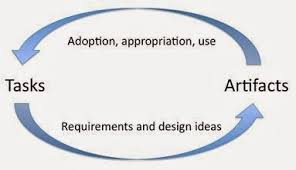
\includegraphics[scale=0.75]{../mci-zusammenfassung/res/task-artifact-cycle.jpeg}
		\end{figure}
	
		\subsubsection*{Examples}
			\begin{enumerate}
				\item Cellphones: Desire to communicate $ \rightarrow $ phone $ \rightarrow $ changed social behavior
				\item Cars: Need for transportation $ \rightarrow $ car $ \rightarrow $ changed mobility behavior \biglb
			\end{enumerate}
	
	
	
	\subsection{Utility, Usability, Likeability}
		\subsubsection*{Utility}
			a product can be used to reach a certain goal or to perform a certain task. This is	essential!

			
		\subsubsection*{Usabiltiy}
			relates to the question of quality and efficiency. E.g. how well does a product	support the user to reach a certain goal or to perform a certain task.
			
		\subsubsection*{Likeability}
			this may be related to utility and usability but not necessarily. People may like a
			product for any other reason\ldots
		